% fig_quad_infeed.tex
% TR-34: Required R_fwd vs k_ibr for different arc resistance values
%
% X-axis: k_ibr [0.05, 0.55]
% Y-axis: R_m = R_arc * (1 + 1/k_ibr) [pu]
%
% Curves for R_arc = 0.004, 0.008, 0.012, 0.020 pu
% Horizontal lines: R_fwd1=0.030, R_fwd2=0.050
% Shaded regions showing what Zone 1 / Zone 2 quad covers

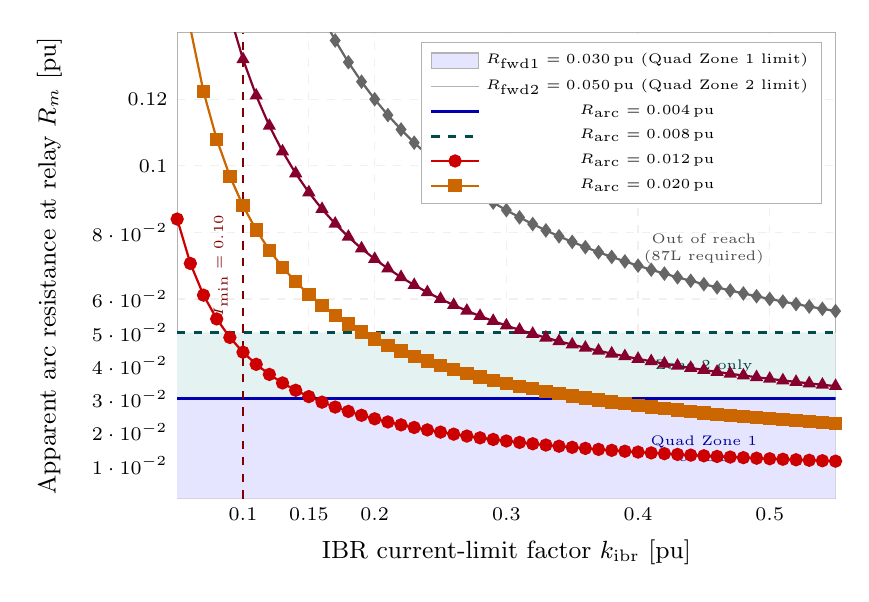
\begin{tikzpicture}
\begin{axis}[
  name        = infax,
  width       = 0.82\textwidth,
  height      = 7.5cm,
  xlabel      = {IBR current-limit factor $k_\mathrm{ibr}$ [pu]},
  ylabel      = {Apparent arc resistance at relay $R_m$ [pu]},
  xlabel style= {font=\small},
  ylabel style= {font=\small, yshift=4pt},
  xmin=0.05, xmax=0.55,
  ymin=0.00, ymax=0.14,
  xtick       = {0.10,0.15,0.20,0.30,0.40,0.50},
  ytick       = {0.01,0.02,0.03,0.04,0.05,0.06,0.08,0.10,0.12},
  xticklabel style={font=\scriptsize},
  yticklabel style={font=\scriptsize},
  grid        = major,
  grid style  = {gray!12, dashed},
  tick style  = {draw=none},
  axis line style={gray!60},
  legend style={at={(0.98,0.98)}, anchor=north east, font=\tiny,
                draw=gray!60, fill=white},
]

%% ── Shaded region: covered by Quad Zone 1 (R_m <= 0.030) ────────────────────
\addplot[fill=blue!10, draw=none, area legend]
  coordinates {(0.05,0) (0.55,0) (0.55,0.030) (0.05,0.030)} \closedcycle;

%% ── Shaded region: covered by Quad Zone 2 only (0.030 < R_m <= 0.050) ────────
\addplot[fill=teal!10, draw=none]
  coordinates {(0.05,0.030) (0.55,0.030) (0.55,0.050) (0.05,0.050)} \closedcycle;

%% ── R_fwd1 and R_fwd2 lines ──────────────────────────────────────────────────
\addplot[blue!70!black, very thick, mark=none]
  coordinates {(0.05,0.030) (0.55,0.030)};
\addlegendentry{$R_\mathrm{fwd1}=0.030$\,pu (Quad Zone~1 limit)}

\addplot[teal!60!black, very thick, dashed, mark=none]
  coordinates {(0.05,0.050) (0.55,0.050)};
\addlegendentry{$R_\mathrm{fwd2}=0.050$\,pu (Quad Zone~2 limit)}

%% ── R_m curves ───────────────────────────────────────────────────────────────
\addplot[red!80!black, thick, mark=*, mark size=2pt,
         domain=0.05:0.55, samples=51]
  ({x}, {0.004*(1+1/x)});
\addlegendentry{$R_\mathrm{arc}=0.004$\,pu}

\addplot[orange!80!black, thick, mark=square*, mark size=2pt,
         domain=0.05:0.55, samples=51]
  ({x}, {0.008*(1+1/x)});
\addlegendentry{$R_\mathrm{arc}=0.008$\,pu}

\addplot[purple!70!black, thick, mark=triangle*, mark size=2pt,
         domain=0.05:0.55, samples=51]
  ({x}, {0.012*(1+1/x)});
\addlegendentry{$R_\mathrm{arc}=0.012$\,pu}

\addplot[black!60, thick, mark=diamond*, mark size=2pt,
         domain=0.05:0.55, samples=51]
  ({x}, {0.020*(1+1/x)});
\addlegendentry{$R_\mathrm{arc}=0.020$\,pu}

%% ── Coverage region labels ───────────────────────────────────────────────────
\node[blue!60!black, font=\tiny, align=center]
  at (axis cs:0.45, 0.015) {Quad Zone~1\\covers};

\node[teal!50!black, font=\tiny, align=center]
  at (axis cs:0.45, 0.040) {Zone~2 only};

\node[gray!60!black, font=\tiny, align=center]
  at (axis cs:0.45, 0.075) {Out of reach\\(87L required)};

%% ── I_min annotation ─────────────────────────────────────────────────────────
\addplot[red!50!black, thin, dashed, mark=none]
  coordinates {(0.10, 0) (0.10, 0.14)};
\node[red!50!black, font=\tiny, rotate=90, above=2pt]
  at (axis cs:0.10, 0.07) {$I_\mathrm{min}=0.10$};

\end{axis}
\end{tikzpicture}
